\documentclass[11pt,a4paper]{article}
\newcommand{\intestazione}{Trimero ad anello --- 5. Il modello di rumore}
% =====================================================================
%  Preambolo comune ai documenti sul dimero (serie "che cosa abbiamo fatto")
%  Incluso con % =====================================================================
%  Preambolo comune ai documenti sul dimero (serie "che cosa abbiamo fatto")
%  Incluso con % =====================================================================
%  Preambolo comune ai documenti sul dimero (serie "che cosa abbiamo fatto")
%  Incluso con \input{preambolo_dimero} subito dopo \documentclass.
% =====================================================================
\usepackage[T1]{fontenc}
\usepackage[utf8]{inputenc}
\usepackage[main=italian,provide=*]{babel}
\usepackage{amsmath,amssymb,mathtools}
\usepackage{graphicx}
\usepackage{booktabs}
\usepackage{colortbl}
\usepackage{xcolor}
\usepackage{geometry}
\usepackage{placeins}
\usepackage{caption}
\usepackage{enumitem}
\usepackage{fancyhdr}
\usepackage{needspace}
\usepackage{tikz}
\usetikzlibrary{arrows.meta,positioning,shapes.geometric,calc,fit,backgrounds}
\usepackage{hyperref}
\hypersetup{colorlinks=true,linkcolor=blu,citecolor=blu,urlcolor=blu}

\geometry{margin=2.5cm}

% --- colori coerenti con quelli delle figure (palette Okabe-Ito)
\definecolor{blu}{HTML}{0072B2}
\definecolor{arancio}{HTML}{E69F00}
\definecolor{verdes}{HTML}{009E73}
\definecolor{rossos}{HTML}{D55E00}
\definecolor{violas}{HTML}{CC79A7}
\definecolor{grigetto}{HTML}{E8E8E8}

\captionsetup{font=small,labelfont=bf,width=0.92\textwidth}

\pagestyle{fancy}
\fancyhf{}
\fancyhead[L]{\small\itshape\intestazione}
\fancyhead[R]{\small\thepage}
\renewcommand{\headrulewidth}{0.3pt}

% --- notazione
\newcommand{\ket}[1]{\lvert #1\rangle}
\newcommand{\bra}[1]{\langle #1 \rvert}
\newcommand{\media}[1]{\langle #1 \rangle}
\newcommand{\vs}[1]{\mathbf{s}_{#1}}

% --- riquadro "in una riga": il messaggio da portare a casa
\newcommand{\messaggio}[1]{%
  \begin{center}
  \begin{minipage}{0.93\textwidth}
  \setlength{\fboxsep}{9pt}%
  \colorbox{grigetto}{\begin{minipage}{\dimexpr\textwidth-2\fboxsep}
  \small\textbf{In una riga.}\enspace #1
  \end{minipage}}
  \end{minipage}
  \end{center}
}

% --- riquadro "come lo sappiamo": la verifica numerica dietro un'affermazione
\newcommand{\verifica}[1]{%
  \begin{center}
  \begin{minipage}{0.93\textwidth}
  \small\textcolor{verdes}{\rule{2.2em}{1.1pt}}\enspace
  \textcolor{verdes}{\textbf{Come lo sappiamo.}}\enspace #1
  \end{minipage}
  \end{center}
  \medskip
}
 subito dopo \documentclass.
% =====================================================================
\usepackage[T1]{fontenc}
\usepackage[utf8]{inputenc}
\usepackage[main=italian,provide=*]{babel}
\usepackage{amsmath,amssymb,mathtools}
\usepackage{graphicx}
\usepackage{booktabs}
\usepackage{colortbl}
\usepackage{xcolor}
\usepackage{geometry}
\usepackage{placeins}
\usepackage{caption}
\usepackage{enumitem}
\usepackage{fancyhdr}
\usepackage{needspace}
\usepackage{tikz}
\usetikzlibrary{arrows.meta,positioning,shapes.geometric,calc,fit,backgrounds}
\usepackage{hyperref}
\hypersetup{colorlinks=true,linkcolor=blu,citecolor=blu,urlcolor=blu}

\geometry{margin=2.5cm}

% --- colori coerenti con quelli delle figure (palette Okabe-Ito)
\definecolor{blu}{HTML}{0072B2}
\definecolor{arancio}{HTML}{E69F00}
\definecolor{verdes}{HTML}{009E73}
\definecolor{rossos}{HTML}{D55E00}
\definecolor{violas}{HTML}{CC79A7}
\definecolor{grigetto}{HTML}{E8E8E8}

\captionsetup{font=small,labelfont=bf,width=0.92\textwidth}

\pagestyle{fancy}
\fancyhf{}
\fancyhead[L]{\small\itshape\intestazione}
\fancyhead[R]{\small\thepage}
\renewcommand{\headrulewidth}{0.3pt}

% --- notazione
\newcommand{\ket}[1]{\lvert #1\rangle}
\newcommand{\bra}[1]{\langle #1 \rvert}
\newcommand{\media}[1]{\langle #1 \rangle}
\newcommand{\vs}[1]{\mathbf{s}_{#1}}

% --- riquadro "in una riga": il messaggio da portare a casa
\newcommand{\messaggio}[1]{%
  \begin{center}
  \begin{minipage}{0.93\textwidth}
  \setlength{\fboxsep}{9pt}%
  \colorbox{grigetto}{\begin{minipage}{\dimexpr\textwidth-2\fboxsep}
  \small\textbf{In una riga.}\enspace #1
  \end{minipage}}
  \end{minipage}
  \end{center}
}

% --- riquadro "come lo sappiamo": la verifica numerica dietro un'affermazione
\newcommand{\verifica}[1]{%
  \begin{center}
  \begin{minipage}{0.93\textwidth}
  \small\textcolor{verdes}{\rule{2.2em}{1.1pt}}\enspace
  \textcolor{verdes}{\textbf{Come lo sappiamo.}}\enspace #1
  \end{minipage}
  \end{center}
  \medskip
}
 subito dopo \documentclass.
% =====================================================================
\usepackage[T1]{fontenc}
\usepackage[utf8]{inputenc}
\usepackage[main=italian,provide=*]{babel}
\usepackage{amsmath,amssymb,mathtools}
\usepackage{graphicx}
\usepackage{booktabs}
\usepackage{colortbl}
\usepackage{xcolor}
\usepackage{geometry}
\usepackage{placeins}
\usepackage{caption}
\usepackage{enumitem}
\usepackage{fancyhdr}
\usepackage{needspace}
\usepackage{tikz}
\usetikzlibrary{arrows.meta,positioning,shapes.geometric,calc,fit,backgrounds}
\usepackage{hyperref}
\hypersetup{colorlinks=true,linkcolor=blu,citecolor=blu,urlcolor=blu}

\geometry{margin=2.5cm}

% --- colori coerenti con quelli delle figure (palette Okabe-Ito)
\definecolor{blu}{HTML}{0072B2}
\definecolor{arancio}{HTML}{E69F00}
\definecolor{verdes}{HTML}{009E73}
\definecolor{rossos}{HTML}{D55E00}
\definecolor{violas}{HTML}{CC79A7}
\definecolor{grigetto}{HTML}{E8E8E8}

\captionsetup{font=small,labelfont=bf,width=0.92\textwidth}

\pagestyle{fancy}
\fancyhf{}
\fancyhead[L]{\small\itshape\intestazione}
\fancyhead[R]{\small\thepage}
\renewcommand{\headrulewidth}{0.3pt}

% --- notazione
\newcommand{\ket}[1]{\lvert #1\rangle}
\newcommand{\bra}[1]{\langle #1 \rvert}
\newcommand{\media}[1]{\langle #1 \rangle}
\newcommand{\vs}[1]{\mathbf{s}_{#1}}

% --- riquadro "in una riga": il messaggio da portare a casa
\newcommand{\messaggio}[1]{%
  \begin{center}
  \begin{minipage}{0.93\textwidth}
  \setlength{\fboxsep}{9pt}%
  \colorbox{grigetto}{\begin{minipage}{\dimexpr\textwidth-2\fboxsep}
  \small\textbf{In una riga.}\enspace #1
  \end{minipage}}
  \end{minipage}
  \end{center}
}

% --- riquadro "come lo sappiamo": la verifica numerica dietro un'affermazione
\newcommand{\verifica}[1]{%
  \begin{center}
  \begin{minipage}{0.93\textwidth}
  \small\textcolor{verdes}{\rule{2.2em}{1.1pt}}\enspace
  \textcolor{verdes}{\textbf{Come lo sappiamo.}}\enspace #1
  \end{minipage}
  \end{center}
  \medskip
}

\providecommand{\Tr}{\operatorname{Tr}}

\title{\bfseries Da $\ket{\psi}$ a $\rho$: mettere un rumore vero nella pipeline\\[2pt]
\large Documento 5 --- il modello di rumore, riusato dal dimero}
\author{Samuele Schiavi \\ \small Tesi triennale in Fisica, Università di Parma
--- Relatore: Prof.\ Alessandro Chiesa}
\date{}

\begin{document}
\maketitle
\thispagestyle{fancy}

\section{Perché il sistema chiuso non basta più}

Tutta la Parte 1 di questa topologia assume un vettore di stato che evolve
in modo perfettamente unitario. Su hardware reale nessuna delle due cose è
vera: ogni gate ha un errore, e la misura stessa non è affidabile al
cento per cento. Serve un formalismo che descriva stati imperfettamente
noti --- l'operatore densità $\rho$ --- e un modello di come il rumore lo
trasforma.

\section{Il cambio di formalismo}

Uno stato puro $\ket\psi$ diventa $\rho=\ket\psi\bra\psi$; sotto un canale
di rumore $\mathcal N$, $\rho\to\mathcal N(\rho)$, in generale non più uno
stato puro. Le osservabili non cambiano forma
($\langle O\rangle=\Tr[\rho O]$), ma $\rho$ porta ora meno informazione di
un vettore di stato --- è il prezzo del rumore.

\section{Due canali, non uno stack di rumore generico}

Confermato dal relatore per l'intera Parte 2 (dimero e trimero
indistintamente): \textbf{solo due canali}, non un modello generico di
rumore hardware.

\begin{itemize}[leftmargin=1.8em,itemsep=3pt]
\item \textbf{Depolarizzante di gate}, a 1 e 2 qubit --- ogni porta
applicata, sul registro a tre qubit come sull'ancilla, porta con sé una
probabilità di errore.
\item \textbf{Readout simmetrico} (come punto di partenza; l'estensione
facoltativa del Documento 11 lo generalizza).
\end{itemize}
$T_1$ e $T_2$ restano esclusi, per la stessa decisione già presa sul
dimero.

\section{Calibrazione: lo stesso chip del dimero}

\begin{table}[htbp]
\centering
\small
\renewcommand{\arraystretch}{1.3}
\begin{tabular}{@{}lc@{}}
\toprule
\rowcolor{grigetto}
\textbf{Parametro} & \textbf{Valore (mediane \texttt{ibm\_torino})} \\
\midrule
$\varepsilon_{1q}$ (gate a 1 qubit) & $2.9\times10^{-4}$ \\
$\varepsilon_{2q}$ (gate a 2 qubit) & $3.8\times10^{-3}$ \\
$p_\text{readout}$ & $2.3\times10^{-2}$ \\
\bottomrule
\end{tabular}
\caption{Stessa calibrazione reale già usata per il dimero (arXiv:2504.15187)
--- non una nuova ricerca: il modello di rumore non dipende dal numero di
qubit del circuito a cui viene applicato, verificato esplicitamente al
momento di aprire questa Parte 2 sull'anello.}
\end{table}
\FloatBarrier

\begin{figure}[htbp]
\centering
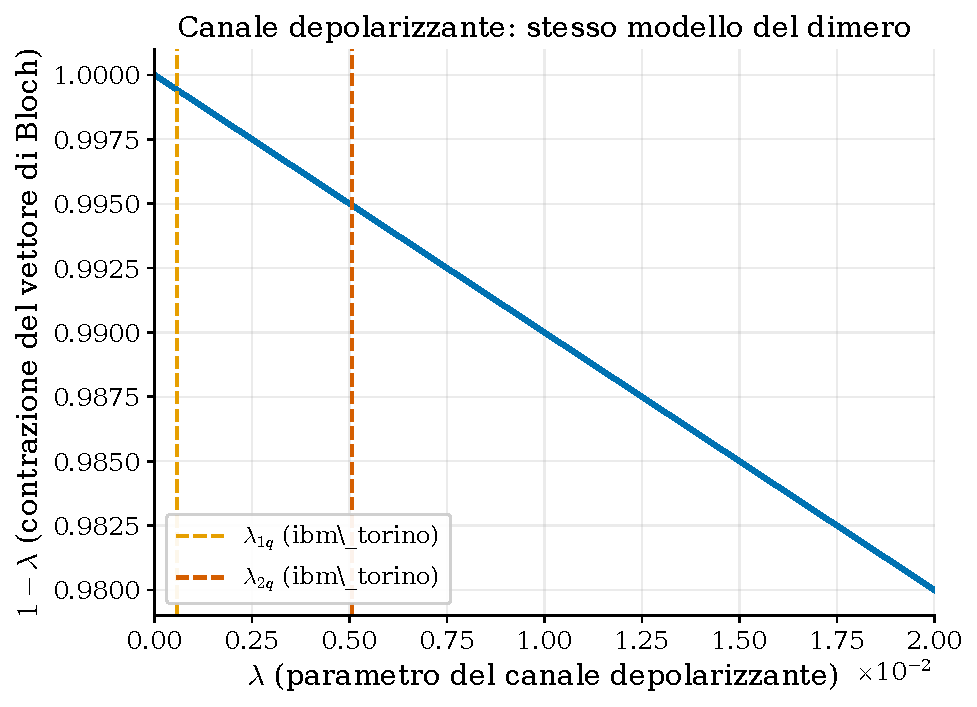
\includegraphics[width=0.62\textwidth]{figure/fig_depolarizzazione_bloch_anello}
\caption{Contrazione della sfera di Bloch sotto il canale depolarizzante,
$1-\lambda$ in funzione di $\lambda$. Le linee verticali segnano i valori
di calibrazione: $\lambda_{1q}=5.80\times10^{-4}$,
$\lambda_{2q}=5.07\times10^{-3}$ --- identici a quelli usati sul dimero,
stessa formula $\lambda_{1q}=2\varepsilon_{1q}$,
$\lambda_{2q}=\tfrac43\varepsilon_{2q}$.}
\end{figure}
\FloatBarrier

\verifica{Il modulo di rumore per l'anello (\texttt{noise\_model\_trimero\_
anello.py}) non ridefinisce nulla: importa e riespone \texttt{build\_noise\_
model} dal dimero. L'operazione che costruisce il \texttt{NoiseModel}
(\texttt{add\_all\_qubit\_quantum\_error}) è per costruzione indipendente
dal numero di qubit del circuito su cui verrà applicata --- non serve una
verifica numerica per ogni nuova topologia, la garanzia è nella struttura
dell'API di Qiskit stessa.}

\section{Cosa resta fuori, dichiarato}

\begin{itemize}[leftmargin=1.5em,itemsep=2pt]
\item Nessun modello di crosstalk fra qubit vicini.
\item Nessuna dipendenza spaziale del rumore (stesso $\varepsilon$ su ogni
qubit e coppia di qubit) --- una semplificazione, non una misura di un chip
specifico qubit per qubit.
\item Il rumore di lettura, in questo documento, resta simmetrico: la sua
generalizzazione è il Documento 11, non qui.
\end{itemize}

\end{document}
